\documentclass[11pt]{article}
\usepackage{graphicx}
\usepackage{geometry}
\usepackage{hyperref}

\begin{document}

\section{Introduction}
Explained by Satoshi Nakamoto in 2008, with a paper about Bitcoin, the Blockchain is grounded on two technologies: asymetric cryptography and distributed systems. There is already a substantial number of blockchain-based applications related to diverse fields such as finance, integrity verification, governance, citizenship, user services, public sector, voting, internet of things, healthcare management, privacy and security, business and industry, supply chain, energy sector, education, data management.\cite{1} \\
The well-known Bitcoin is just one use case of the blockchain technology. There is a whole world beyond cryptocurrency that could benefit from the unique confluence of smart contracts and smart devices.\\
Smart-contracts are user-defined programs or protocols that can be automatically enforced once certain preconditions are met. Those executable programs define rules for writing in the distributed ledger, without the need of any centralized control. Building trust in a distributed environment will change the way we share information, interact with each other and thus do business, especially in the IoT industry.\cite{2}\\
As shown in the following figure\cite{3}, the number of electronic devices around us is always growing, with already more than 7 Billions IoT devices in 2019. A large part of the future growth should come from ow-power wide area networtk (LPWAN), a technology allowing an extremely high battery life and a maximum communication range over 20 kilometers. There is already more than 25 Millions devices -the majority of which are smart meters- connected through LPWAN, and this number should increase to more than 2 Billions devices by 2025.\\
\begin{figure}[h]
	\centering
	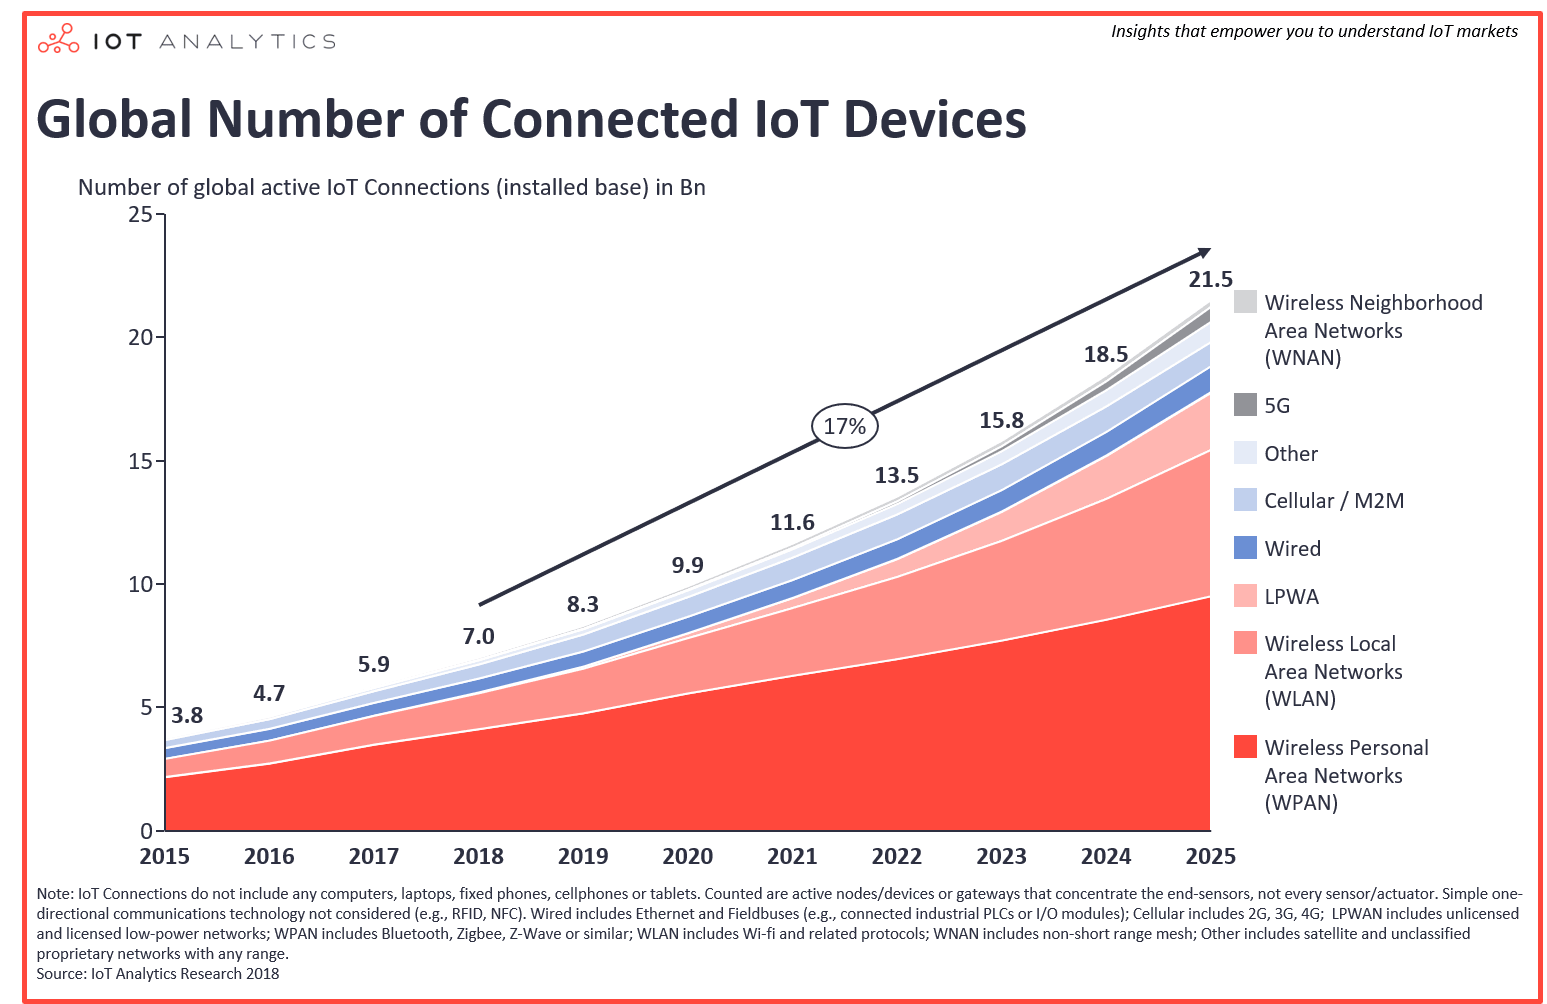
\includegraphics[width=0.8\linewidth]{stateofIoT2018.png}
\end{figure}\\
\\
Smart-meters allows to monitor electric energy consumption. These data can be transmitted to energy suppliers for billing. Although a large amount of data provided by smart devices -like the ones recorded by smaart-meters- could be used to adequately adjust energy consumption and/or optimize networks, it may also raise critical privacy issues,\cite{4} that the Blockchain technology might be able to solve.

\section{Literature review}
4 pages\\
ML.\,Achart expected 22.02.2019

\section{Presentation of our solution (6pages)}
\subsection{our solution concept (1page)}
\subsection{our solution design: architecture, module, code abstracts...(4pages)}
\subsection{our solution evaluation: features, bugs...(1page)}
blockchain for social impact: methodology from \textit{Stanford Business School, Center for Social Innovation, 2018, Blockchain For Social Impact Moving Beyond The Hype}:\\
1-what is the problem of your organization is trying to solve? What are your end users?\\
2-How does your initiative use blockchain, and why is blockchain a good technology for this problem?\\
3-What technologies or services are available to solve this problem, and how is blockchain a better solution?\\
4-what is your initiative's intended impact? How do you measure it?\\
5-In what time do you think you will see meaningful impact from your blockchain initiative?\\

\section{Conclusion}
3pages\\
ML.\,Achart expected 22.02.2019

\begin{thebibliography}{9}

\bibitem{1}
	Fran Casino, Thomas K.\,Dasaklis, Constantinos Patsakis,
	\textit{A systematic literature review of blockchain-based applications: Current status, classification and open issues},
	\hyperref[https://doi.org/10.1016/j.tele.2018.11.006]{https://doi.org/10.1016/j.tele.2018.11.006}
\bibitem{2}
	Ana Reyna, Cristian Martín, Jaime Chen, Enrique Soler, Manuel Díaz,
	\textit{On blockchain and its integration with IoT. Challenges and opportunities}
	\hyperref[https://doi.org/10.1016/j.future.2018.05.046]{https://doi.org/10.1016/j.future.2018.05.046}
\bibitem{3}
	Knud Lasse Lueth,
	\textit{State of the IoT 2018: Number of IoT devices now at 7B – Market accelerating}
	\hyperref[https://iot-analytics.com/state-of-the-iot-update-q1-q2-2018-number-of-iot-devices-now-7b/]{https://iot-analytics.com/state-of-the-iot-update-q1-q2-2018-number-of-iot-devices-now-7b/}
\bibitem{4}
	Marco Conoscenti, Antonio Vetrò, Juan Carlos De Martin
	\textit{Blockchain for the Internet of Things: a Systematic Literature Review}
	\hyperref[https://ieeexplore.ieee.org/abstract/document/7945805]{https://ieeexplore.ieee.org/abstract/document/7945805}
\bibitem{5}
	aut
	\textit{tit}
	\hyperref[]{}
\bibitem{6}
	aut
	\textit{tit}
	\hyperref[]{}
\bibitem{7}
	aut
	\textit{tit}
	\hyperref[]{}
\bibitem{8}
	aut
	\textit{tit}
	\hyperref[]{}



\end{thebibliography}

	
\end{document}